\documentclass[twoside]{book}

% Packages required by doxygen
\usepackage{calc}
\usepackage{doxygen}
\usepackage{graphicx}
\usepackage[utf8]{inputenc}
\usepackage{makeidx}
\usepackage{multicol}
\usepackage{multirow}
\usepackage{textcomp}
\usepackage[table]{xcolor}

% Font selection
\usepackage[T1]{fontenc}
\usepackage{mathptmx}
\usepackage[scaled=.90]{helvet}
\usepackage{courier}
\usepackage{amssymb}
\usepackage{sectsty}
\renewcommand{\familydefault}{\sfdefault}
\allsectionsfont{%
  \fontseries{bc}\selectfont%
  \color{darkgray}%
}
\renewcommand{\DoxyLabelFont}{%
  \fontseries{bc}\selectfont%
  \color{darkgray}%
}

% Page & text layout
\usepackage{geometry}
\geometry{%
  a4paper,%
  top=2.5cm,%
  bottom=2.5cm,%
  left=2.5cm,%
  right=2.5cm%
}
\tolerance=750
\hfuzz=15pt
\hbadness=750
\setlength{\emergencystretch}{15pt}
\setlength{\parindent}{0cm}
\setlength{\parskip}{0.2cm}
\makeatletter
\renewcommand{\paragraph}{%
  \@startsection{paragraph}{4}{0ex}{-1.0ex}{1.0ex}{%
    \normalfont\normalsize\bfseries\SS@parafont%
  }%
}
\renewcommand{\subparagraph}{%
  \@startsection{subparagraph}{5}{0ex}{-1.0ex}{1.0ex}{%
    \normalfont\normalsize\bfseries\SS@subparafont%
  }%
}
\makeatother

% Headers & footers
\usepackage{fancyhdr}
\pagestyle{fancyplain}
\fancyhead[LE]{\fancyplain{}{\bfseries\thepage}}
\fancyhead[CE]{\fancyplain{}{}}
\fancyhead[RE]{\fancyplain{}{\bfseries\leftmark}}
\fancyhead[LO]{\fancyplain{}{\bfseries\rightmark}}
\fancyhead[CO]{\fancyplain{}{}}
\fancyhead[RO]{\fancyplain{}{\bfseries\thepage}}
\fancyfoot[LE]{\fancyplain{}{}}
\fancyfoot[CE]{\fancyplain{}{}}
\fancyfoot[RE]{\fancyplain{}{\bfseries\scriptsize Generated on Mon Mar 11 2019 10\-:28\-:49 for My Project by Doxygen }}
\fancyfoot[LO]{\fancyplain{}{\bfseries\scriptsize Generated on Mon Mar 11 2019 10\-:28\-:49 for My Project by Doxygen }}
\fancyfoot[CO]{\fancyplain{}{}}
\fancyfoot[RO]{\fancyplain{}{}}
\renewcommand{\footrulewidth}{0.4pt}
\renewcommand{\chaptermark}[1]{%
  \markboth{#1}{}%
}
\renewcommand{\sectionmark}[1]{%
  \markright{\thesection\ #1}%
}

% Indices & bibliography
\usepackage{natbib}
\usepackage[titles]{tocloft}
\setcounter{tocdepth}{3}
\setcounter{secnumdepth}{5}
\makeindex

% Hyperlinks (required, but should be loaded last)
\usepackage{ifpdf}
\ifpdf
  \usepackage[pdftex,pagebackref=true]{hyperref}
\else
  \usepackage[ps2pdf,pagebackref=true]{hyperref}
\fi
\hypersetup{%
  colorlinks=true,%
  linkcolor=blue,%
  citecolor=blue,%
  unicode%
}

% Custom commands
\newcommand{\clearemptydoublepage}{%
  \newpage{\pagestyle{empty}\cleardoublepage}%
}


%===== C O N T E N T S =====

\begin{document}

% Titlepage & ToC
\hypersetup{pageanchor=false}
\pagenumbering{roman}
\begin{titlepage}
\vspace*{7cm}
\begin{center}%
{\Large My Project }\\
\vspace*{1cm}
{\large Generated by Doxygen 1.8.5}\\
\vspace*{0.5cm}
{\small Mon Mar 11 2019 10:28:49}\\
\end{center}
\end{titlepage}
\clearemptydoublepage
\tableofcontents
\clearemptydoublepage
\pagenumbering{arabic}
\hypersetup{pageanchor=true}

%--- Begin generated contents ---
\chapter{Hierarchical Index}
\section{Class Hierarchy}
This inheritance list is sorted roughly, but not completely, alphabetically\-:\begin{DoxyCompactList}
\item \contentsline{section}{Black\-Scholes\-Model}{\pageref{classBlackScholesModel}}{}
\item \contentsline{section}{Monte\-Carlo}{\pageref{classMonteCarlo}}{}
\item \contentsline{section}{Option}{\pageref{classOption}}{}
\begin{DoxyCompactList}
\item \contentsline{section}{Asian\-Option}{\pageref{classAsianOption}}{}
\item \contentsline{section}{Basket\-Option}{\pageref{classBasketOption}}{}
\item \contentsline{section}{Call\-Option}{\pageref{classCallOption}}{}
\item \contentsline{section}{Performance\-Option}{\pageref{classPerformanceOption}}{}
\end{DoxyCompactList}
\end{DoxyCompactList}

\chapter{Class Index}
\section{Class List}
Here are the classes, structs, unions and interfaces with brief descriptions\-:\begin{DoxyCompactList}
\item\contentsline{section}{\hyperlink{classAsianOption}{Asian\-Option} \\*\hyperlink{classOption}{Option} Asiatique hérite de la classe abstraite option }{\pageref{classAsianOption}}{}
\item\contentsline{section}{\hyperlink{classBasketOption}{Basket\-Option} \\*\hyperlink{classOption}{Option} Basket hérite de la classe abstraite option }{\pageref{classBasketOption}}{}
\item\contentsline{section}{\hyperlink{classBlackScholesModel}{Black\-Scholes\-Model} \\*Modèle de Black Scholes }{\pageref{classBlackScholesModel}}{}
\item\contentsline{section}{\hyperlink{classCallOption}{Call\-Option} \\*\hyperlink{classOption}{Option} Call hérite de la classe abstraite option }{\pageref{classCallOption}}{}
\item\contentsline{section}{\hyperlink{classMonteCarlo}{Monte\-Carlo} \\*Méthode de Monte Carlo pour les calculs }{\pageref{classMonteCarlo}}{}
\item\contentsline{section}{\hyperlink{classOption}{Option} \\*Classe \hyperlink{classOption}{Option} abstraite }{\pageref{classOption}}{}
\item\contentsline{section}{\hyperlink{classPerformanceOption}{Performance\-Option} \\*\hyperlink{classOption}{Option} Performance hérite de la classe abstraite option }{\pageref{classPerformanceOption}}{}
\end{DoxyCompactList}

\chapter{Class Documentation}
\hypertarget{classAsianOption}{\section{Asian\-Option Class Reference}
\label{classAsianOption}\index{Asian\-Option@{Asian\-Option}}
}


\hyperlink{classOption}{Option} Asiatique hérite de la classe abstraite option.  




{\ttfamily \#include $<$Asian\-Option.\-hpp$>$}

Inheritance diagram for Asian\-Option\-:\begin{figure}[H]
\begin{center}
\leavevmode
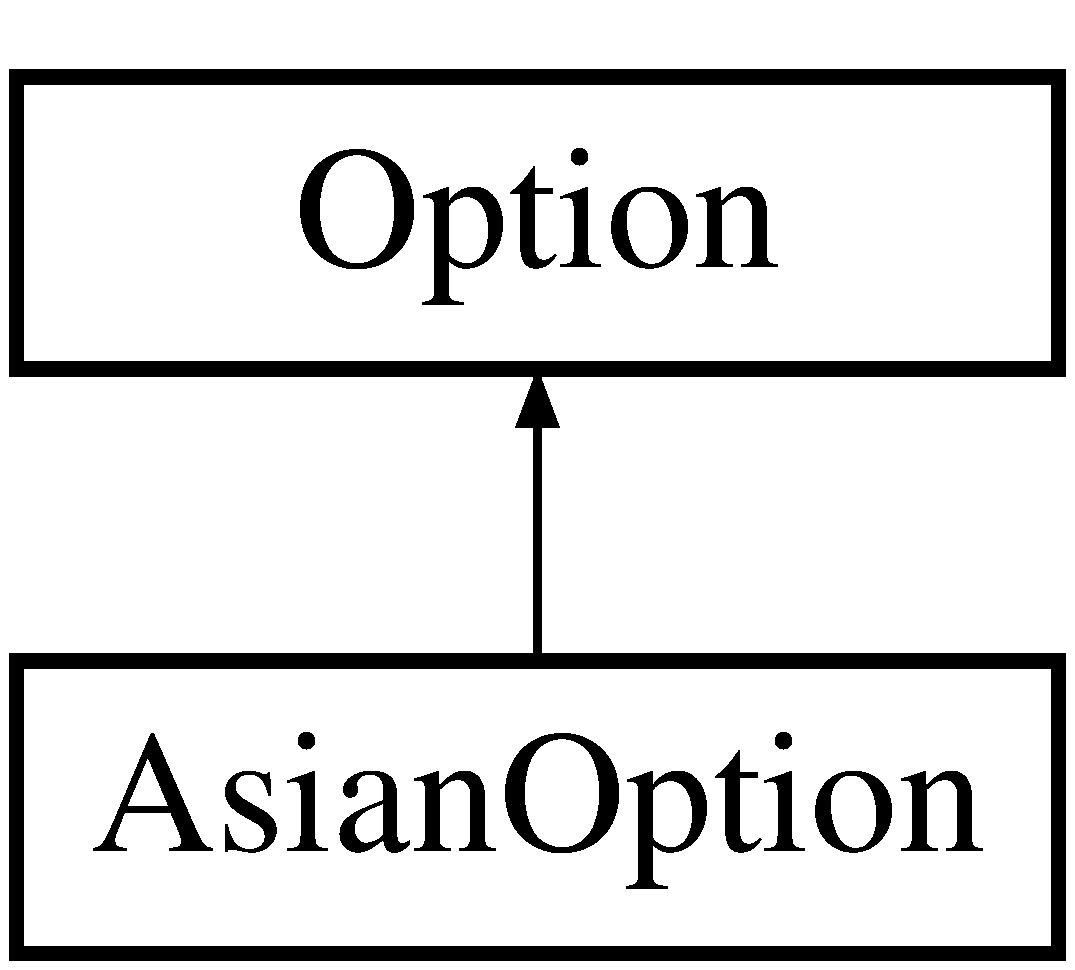
\includegraphics[height=2.000000cm]{classAsianOption}
\end{center}
\end{figure}
\subsection*{Public Member Functions}
\begin{DoxyCompactItemize}
\item 
\hyperlink{classAsianOption_a6e9a45c005716e8e5eec0094b242a615}{Asian\-Option} (double T, int nb\-Time\-Steps, int size, Pnl\-Vect $\ast$weights, double strike)
\item 
double \hyperlink{classAsianOption_a0ac88380a30a7c0ef6a5c5159d15fa76}{payoff} (const Pnl\-Mat $\ast$path) override
\end{DoxyCompactItemize}
\subsection*{Public Attributes}
\begin{DoxyCompactItemize}
\item 
double \hyperlink{classAsianOption_a05e393157001728b21918c8342d7e7e1}{strike\-\_\-}
\end{DoxyCompactItemize}


\subsection{Detailed Description}
\hyperlink{classOption}{Option} Asiatique hérite de la classe abstraite option. 

\subsection{Constructor \& Destructor Documentation}
\hypertarget{classAsianOption_a6e9a45c005716e8e5eec0094b242a615}{\index{Asian\-Option@{Asian\-Option}!Asian\-Option@{Asian\-Option}}
\index{Asian\-Option@{Asian\-Option}!AsianOption@{Asian\-Option}}
\subsubsection[{Asian\-Option}]{\setlength{\rightskip}{0pt plus 5cm}Asian\-Option\-::\-Asian\-Option (
\begin{DoxyParamCaption}
\item[{double}]{T, }
\item[{int}]{nb\-Time\-Steps, }
\item[{int}]{size, }
\item[{Pnl\-Vect $\ast$}]{weights, }
\item[{double}]{strike}
\end{DoxyParamCaption}
)}}\label{classAsianOption_a6e9a45c005716e8e5eec0094b242a615}
Constructeur de la classe 
\begin{DoxyParams}[1]{Parameters}
\mbox{\tt in}  & {\em T} & \-: maturité \\
\hline
\mbox{\tt in}  & {\em nb\-Time\-Steps} & \-: nombre de pas de temps de discrétisation \\
\hline
\mbox{\tt in}  & {\em size} & \-: dimension du modèle \\
\hline
\mbox{\tt in}  & {\em weights} & \-: poids des actifs \\
\hline
\mbox{\tt in}  & {\em strike} & \-: prix d'exercice de l'option \\
\hline
\end{DoxyParams}


\subsection{Member Function Documentation}
\hypertarget{classAsianOption_a0ac88380a30a7c0ef6a5c5159d15fa76}{\index{Asian\-Option@{Asian\-Option}!payoff@{payoff}}
\index{payoff@{payoff}!AsianOption@{Asian\-Option}}
\subsubsection[{payoff}]{\setlength{\rightskip}{0pt plus 5cm}double Asian\-Option\-::payoff (
\begin{DoxyParamCaption}
\item[{const Pnl\-Mat $\ast$}]{path}
\end{DoxyParamCaption}
)\hspace{0.3cm}{\ttfamily [override]}, {\ttfamily [virtual]}}}\label{classAsianOption_a0ac88380a30a7c0ef6a5c5159d15fa76}
Calcule la valeur du payoff sur la trajectoire


\begin{DoxyParams}[1]{Parameters}
\mbox{\tt in}  & {\em path} & est une matrice de taille (N+1) x d contenant une trajectoire du modèle telle que créée par la fonction asset. \\
\hline
\end{DoxyParams}
\begin{DoxyReturn}{Returns}
phi(trajectoire) 
\end{DoxyReturn}


Implements \hyperlink{classOption_abe90882a11f5436077425249e3f32204}{Option}.



\subsection{Member Data Documentation}
\hypertarget{classAsianOption_a05e393157001728b21918c8342d7e7e1}{\index{Asian\-Option@{Asian\-Option}!strike\-\_\-@{strike\-\_\-}}
\index{strike\-\_\-@{strike\-\_\-}!AsianOption@{Asian\-Option}}
\subsubsection[{strike\-\_\-}]{\setlength{\rightskip}{0pt plus 5cm}double Asian\-Option\-::strike\-\_\-}}\label{classAsianOption_a05e393157001728b21918c8342d7e7e1}
Prix d'exercice de l'option asiatique 

The documentation for this class was generated from the following files\-:\begin{DoxyCompactItemize}
\item 
/user/5/.\-base/mazarsa/home/3a/calcul\-\_\-parallèle/projet/pricer/chamilo/pricer-\/skel/src/Asian\-Option.\-hpp\item 
/user/5/.\-base/mazarsa/home/3a/calcul\-\_\-parallèle/projet/pricer/chamilo/pricer-\/skel/src/Asian\-Option.\-cpp\end{DoxyCompactItemize}

\hypertarget{classBasketOption}{\section{Basket\-Option Class Reference}
\label{classBasketOption}\index{Basket\-Option@{Basket\-Option}}
}


\hyperlink{classOption}{Option} Basket hérite de la classe abstraite option.  




{\ttfamily \#include $<$Basket\-Option.\-hpp$>$}

Inheritance diagram for Basket\-Option\-:\begin{figure}[H]
\begin{center}
\leavevmode
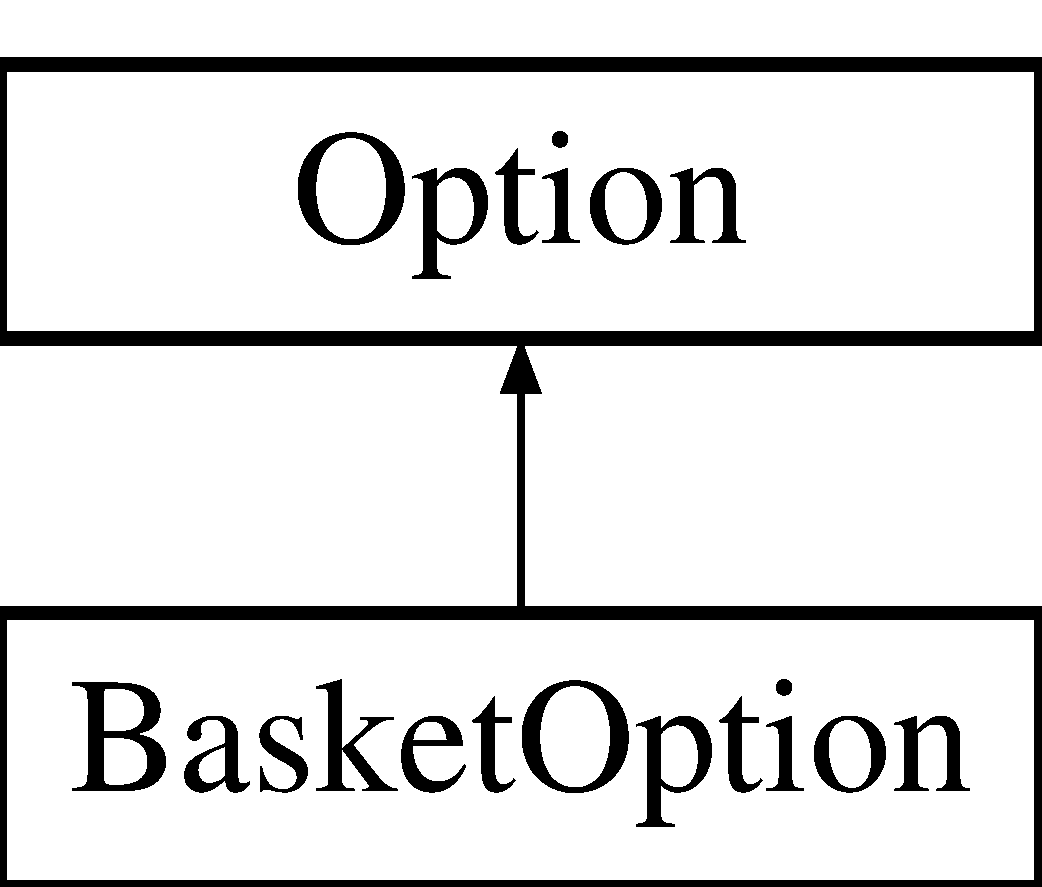
\includegraphics[height=2.000000cm]{classBasketOption}
\end{center}
\end{figure}
\subsection*{Public Member Functions}
\begin{DoxyCompactItemize}
\item 
\hyperlink{classBasketOption_a1842966514887a4e9086ec5ffb176558}{Basket\-Option} (double T, int nb\-Time\-Steps, int size, Pnl\-Vect $\ast$weights, double strike)
\item 
double \hyperlink{classBasketOption_a57c941403d2bd21159b090fa6481ee9e}{payoff} (const Pnl\-Mat $\ast$path) override
\end{DoxyCompactItemize}
\subsection*{Public Attributes}
\begin{DoxyCompactItemize}
\item 
double \hyperlink{classBasketOption_abf96256c30b8e0d063611b11972d32c5}{strike\-\_\-}
\end{DoxyCompactItemize}


\subsection{Detailed Description}
\hyperlink{classOption}{Option} Basket hérite de la classe abstraite option. 

\subsection{Constructor \& Destructor Documentation}
\hypertarget{classBasketOption_a1842966514887a4e9086ec5ffb176558}{\index{Basket\-Option@{Basket\-Option}!Basket\-Option@{Basket\-Option}}
\index{Basket\-Option@{Basket\-Option}!BasketOption@{Basket\-Option}}
\subsubsection[{Basket\-Option}]{\setlength{\rightskip}{0pt plus 5cm}Basket\-Option\-::\-Basket\-Option (
\begin{DoxyParamCaption}
\item[{double}]{T, }
\item[{int}]{nb\-Time\-Steps, }
\item[{int}]{size, }
\item[{Pnl\-Vect $\ast$}]{weights, }
\item[{double}]{strike}
\end{DoxyParamCaption}
)}}\label{classBasketOption_a1842966514887a4e9086ec5ffb176558}
Constructeur de la classe 
\begin{DoxyParams}[1]{Parameters}
\mbox{\tt in}  & {\em T} & \-: maturité \\
\hline
\mbox{\tt in}  & {\em nb\-Time\-Steps} & \-: nombre de pas de temps de discrétisation \\
\hline
\mbox{\tt in}  & {\em size} & \-: dimension du modèle \\
\hline
\mbox{\tt in}  & {\em weights} & \-: poids des actifs \\
\hline
\mbox{\tt in}  & {\em strike} & \-: prix d'exercice de l'option \\
\hline
\end{DoxyParams}


\subsection{Member Function Documentation}
\hypertarget{classBasketOption_a57c941403d2bd21159b090fa6481ee9e}{\index{Basket\-Option@{Basket\-Option}!payoff@{payoff}}
\index{payoff@{payoff}!BasketOption@{Basket\-Option}}
\subsubsection[{payoff}]{\setlength{\rightskip}{0pt plus 5cm}double Basket\-Option\-::payoff (
\begin{DoxyParamCaption}
\item[{const Pnl\-Mat $\ast$}]{path}
\end{DoxyParamCaption}
)\hspace{0.3cm}{\ttfamily [override]}, {\ttfamily [virtual]}}}\label{classBasketOption_a57c941403d2bd21159b090fa6481ee9e}
Calcule la valeur du payoff sur la trajectoire


\begin{DoxyParams}[1]{Parameters}
\mbox{\tt in}  & {\em path} & est une matrice de taille (N+1) x d contenant une trajectoire du modèle telle que créée par la fonction asset. \\
\hline
\end{DoxyParams}
\begin{DoxyReturn}{Returns}
phi(trajectoire) 
\end{DoxyReturn}


Implements \hyperlink{classOption_abe90882a11f5436077425249e3f32204}{Option}.



\subsection{Member Data Documentation}
\hypertarget{classBasketOption_abf96256c30b8e0d063611b11972d32c5}{\index{Basket\-Option@{Basket\-Option}!strike\-\_\-@{strike\-\_\-}}
\index{strike\-\_\-@{strike\-\_\-}!BasketOption@{Basket\-Option}}
\subsubsection[{strike\-\_\-}]{\setlength{\rightskip}{0pt plus 5cm}double Basket\-Option\-::strike\-\_\-}}\label{classBasketOption_abf96256c30b8e0d063611b11972d32c5}
Prix d'exercice de l'option basket 

The documentation for this class was generated from the following files\-:\begin{DoxyCompactItemize}
\item 
/user/5/.\-base/mazarsa/home/3a/calcul\-\_\-parallèle/projet/pricer/chamilo/pricer-\/skel/src/Basket\-Option.\-hpp\item 
/user/5/.\-base/mazarsa/home/3a/calcul\-\_\-parallèle/projet/pricer/chamilo/pricer-\/skel/src/Basket\-Option.\-cpp\end{DoxyCompactItemize}

\hypertarget{classBlackScholesModel}{\section{Black\-Scholes\-Model Class Reference}
\label{classBlackScholesModel}\index{Black\-Scholes\-Model@{Black\-Scholes\-Model}}
}


Modèle de Black Scholes.  




{\ttfamily \#include $<$Black\-Scholes\-Model.\-hpp$>$}

\subsection*{Public Member Functions}
\begin{DoxyCompactItemize}
\item 
\hyperlink{classBlackScholesModel_a803b1ad2cd281d16f0ac66145dbdc9f3}{Black\-Scholes\-Model} (int size, double r, double rho, Pnl\-Vect $\ast$sigma, Pnl\-Vect $\ast$spot, Pnl\-Vect $\ast$trend)
\item 
void \hyperlink{classBlackScholesModel_a71ed54a0ca9a89b87610ff699814e120}{asset} (Pnl\-Mat $\ast$path, double T, int nb\-Time\-Steps, Pnl\-Rng $\ast$rng)
\item 
void \hyperlink{classBlackScholesModel_a9b2fb8790c28edca5d47c712133af14f}{asset} (Pnl\-Mat $\ast$path, double t, double T, int nb\-Time\-Steps, Pnl\-Rng $\ast$rng, const Pnl\-Mat $\ast$past, double nb\-Steps, int a)
\item 
void \hyperlink{classBlackScholesModel_ac89a165e6d27cc12dd77627597f7f56d}{shift\-Asset} (Pnl\-Mat $\ast$shift\-\_\-path, const Pnl\-Mat $\ast$path, int d, double h, double t, double timestep)
\item 
void \hyperlink{classBlackScholesModel_affbc621fa8678a7aa9aa4699f27f5258}{simul\-\_\-market} (Pnl\-Mat $\ast$simulated\-Market, double T, Pnl\-Rng $\ast$rng)
\end{DoxyCompactItemize}
\subsection*{Public Attributes}
\begin{DoxyCompactItemize}
\item 
int \hyperlink{classBlackScholesModel_ab84e9318c0c1e8a50d5e2f9a70f1256e}{size\-\_\-}
\item 
double \hyperlink{classBlackScholesModel_a9b07eb1d8a7ada20e1a723ba19172644}{r\-\_\-}
\item 
double \hyperlink{classBlackScholesModel_a1022a65929e3656f8990b7b0a63705ba}{rho\-\_\-}
\item 
Pnl\-Vect $\ast$ \hyperlink{classBlackScholesModel_a745a2d85da5056b44bd88f37ee7b33e0}{sigma\-\_\-}
\item 
Pnl\-Vect $\ast$ \hyperlink{classBlackScholesModel_a6ce6853d5f0d65c8e0f07cdedca3e26a}{spot\-\_\-}
\item 
Pnl\-Vect $\ast$ \hyperlink{classBlackScholesModel_af92b535c61f17e7a16af56952739302f}{trend\-\_\-}
\end{DoxyCompactItemize}


\subsection{Detailed Description}
Modèle de Black Scholes. 

\subsection{Constructor \& Destructor Documentation}
\hypertarget{classBlackScholesModel_a803b1ad2cd281d16f0ac66145dbdc9f3}{\index{Black\-Scholes\-Model@{Black\-Scholes\-Model}!Black\-Scholes\-Model@{Black\-Scholes\-Model}}
\index{Black\-Scholes\-Model@{Black\-Scholes\-Model}!BlackScholesModel@{Black\-Scholes\-Model}}
\subsubsection[{Black\-Scholes\-Model}]{\setlength{\rightskip}{0pt plus 5cm}Black\-Scholes\-Model\-::\-Black\-Scholes\-Model (
\begin{DoxyParamCaption}
\item[{int}]{size, }
\item[{double}]{r, }
\item[{double}]{rho, }
\item[{Pnl\-Vect $\ast$}]{sigma, }
\item[{Pnl\-Vect $\ast$}]{spot, }
\item[{Pnl\-Vect $\ast$}]{trend}
\end{DoxyParamCaption}
)}}\label{classBlackScholesModel_a803b1ad2cd281d16f0ac66145dbdc9f3}
Constructeur de la classe 
\begin{DoxyParams}[1]{Parameters}
\mbox{\tt in}  & {\em size} & \-: nombre d'actifs du modèle \\
\hline
\mbox{\tt in}  & {\em r} & \-: taux d'intérêt \\
\hline
\mbox{\tt in}  & {\em rho} & \-: paramètre de corrélation \\
\hline
\mbox{\tt in}  & {\em sigma} & \-: vecteur de volatilités \\
\hline
\mbox{\tt in}  & {\em spot} & \-: valeurs initiales des sous-\/jacents \\
\hline
\mbox{\tt in}  & {\em trend} & \-: tendance du modèle \\
\hline
\end{DoxyParams}


\subsection{Member Function Documentation}
\hypertarget{classBlackScholesModel_a71ed54a0ca9a89b87610ff699814e120}{\index{Black\-Scholes\-Model@{Black\-Scholes\-Model}!asset@{asset}}
\index{asset@{asset}!BlackScholesModel@{Black\-Scholes\-Model}}
\subsubsection[{asset}]{\setlength{\rightskip}{0pt plus 5cm}void Black\-Scholes\-Model\-::asset (
\begin{DoxyParamCaption}
\item[{Pnl\-Mat $\ast$}]{path, }
\item[{double}]{T, }
\item[{int}]{nb\-Time\-Steps, }
\item[{Pnl\-Rng $\ast$}]{rng}
\end{DoxyParamCaption}
)}}\label{classBlackScholesModel_a71ed54a0ca9a89b87610ff699814e120}
Génère une trajectoire du modèle et la stocke dans path


\begin{DoxyParams}[1]{Parameters}
\mbox{\tt out}  & {\em path} & contient une trajectoire du modèle. C'est une matrice de taille (nb\-Time\-Steps+1) x d \\
\hline
\mbox{\tt in}  & {\em T} & maturité \\
\hline
\mbox{\tt in}  & {\em rng} & generateur de nombres aleatoires \\
\hline
\mbox{\tt in}  & {\em nb\-Time\-Steps} & nombre de dates de constatation\\
\hline
\end{DoxyParams}
Génère une trajectoire du modèle et la stocke dans path


\begin{DoxyParams}[1]{Parameters}
\mbox{\tt out}  & {\em path} & contient une trajectoire du modèle. C'est une matrice de taille (nb\-Time\-Steps+1) x d \\
\hline
\mbox{\tt in}  & {\em T} & maturité \\
\hline
\mbox{\tt in}  & {\em nb\-Time\-Steps} & nombre de dates de constatation \\
\hline
\end{DoxyParams}
\hypertarget{classBlackScholesModel_a9b2fb8790c28edca5d47c712133af14f}{\index{Black\-Scholes\-Model@{Black\-Scholes\-Model}!asset@{asset}}
\index{asset@{asset}!BlackScholesModel@{Black\-Scholes\-Model}}
\subsubsection[{asset}]{\setlength{\rightskip}{0pt plus 5cm}void Black\-Scholes\-Model\-::asset (
\begin{DoxyParamCaption}
\item[{Pnl\-Mat $\ast$}]{path, }
\item[{double}]{t, }
\item[{double}]{T, }
\item[{int}]{nb\-Time\-Steps, }
\item[{Pnl\-Rng $\ast$}]{rng, }
\item[{const Pnl\-Mat $\ast$}]{past, }
\item[{double}]{nb\-Steps, }
\item[{int}]{a}
\end{DoxyParamCaption}
)}}\label{classBlackScholesModel_a9b2fb8790c28edca5d47c712133af14f}
Calcule une trajectoire du sous-\/jacent connaissant le passé jusqu' à la date t


\begin{DoxyParams}[1]{Parameters}
\mbox{\tt out}  & {\em path} & contient une trajectoire du sous-\/jacent donnée jusqu'à l'instant t par la matrice past \\
\hline
\mbox{\tt in}  & {\em t} & date jusqu'à laquelle on connait la trajectoire. t n'est pas forcément une date de discrétisation \\
\hline
\mbox{\tt in}  & {\em nb\-Time\-Steps} & nombre de pas de constatation \\
\hline
\mbox{\tt in}  & {\em T} & date jusqu'à laquelle on simule la trajectoire \\
\hline
\mbox{\tt in}  & {\em rng} & generateur de nombres aleatoires \\
\hline
\mbox{\tt in}  & {\em past} & trajectoire réalisée jusqu'a la date t\\
\hline
\end{DoxyParams}
Calcule une trajectoire du sous-\/jacent connaissant le passé jusqu' à la date t


\begin{DoxyParams}[1]{Parameters}
\mbox{\tt out}  & {\em path} & contient une trajectoire du sous-\/jacent donnée jusqu'à l'instant t par la matrice past \\
\hline
\mbox{\tt in}  & {\em t} & date jusqu'à laquelle on connait la trajectoire. t n'est pas forcément une date de discrétisation \\
\hline
\mbox{\tt in}  & {\em nb\-Time\-Steps} & nombre de pas de constatation \\
\hline
\mbox{\tt in}  & {\em T} & date jusqu'à laquelle on simule la trajectoire \\
\hline
\mbox{\tt in}  & {\em past} & trajectoire réalisée jusqu'a la date t \\
\hline
\end{DoxyParams}
\hypertarget{classBlackScholesModel_ac89a165e6d27cc12dd77627597f7f56d}{\index{Black\-Scholes\-Model@{Black\-Scholes\-Model}!shift\-Asset@{shift\-Asset}}
\index{shift\-Asset@{shift\-Asset}!BlackScholesModel@{Black\-Scholes\-Model}}
\subsubsection[{shift\-Asset}]{\setlength{\rightskip}{0pt plus 5cm}void Black\-Scholes\-Model\-::shift\-Asset (
\begin{DoxyParamCaption}
\item[{Pnl\-Mat $\ast$}]{shift\-\_\-path, }
\item[{const Pnl\-Mat $\ast$}]{path, }
\item[{int}]{d, }
\item[{double}]{h, }
\item[{double}]{t, }
\item[{double}]{timestep}
\end{DoxyParamCaption}
)}}\label{classBlackScholesModel_ac89a165e6d27cc12dd77627597f7f56d}
Shift d'une trajectoire du sous-\/jacent


\begin{DoxyParams}[1]{Parameters}
\mbox{\tt in}  & {\em path} & contient en input la trajectoire du sous-\/jacent \\
\hline
\mbox{\tt out}  & {\em shift\-\_\-path} & contient la trajectoire path dont la composante d a été shiftée par (1+h) à partir de la date t. \\
\hline
\mbox{\tt in}  & {\em t} & date à partir de laquelle on shift \\
\hline
\mbox{\tt in}  & {\em h} & pas de différences finies \\
\hline
\mbox{\tt in}  & {\em d} & indice du sous-\/jacent à shifter \\
\hline
\mbox{\tt in}  & {\em timestep} & pas de constatation du sous-\/jacent \\
\hline
\end{DoxyParams}
\hypertarget{classBlackScholesModel_affbc621fa8678a7aa9aa4699f27f5258}{\index{Black\-Scholes\-Model@{Black\-Scholes\-Model}!simul\-\_\-market@{simul\-\_\-market}}
\index{simul\-\_\-market@{simul\-\_\-market}!BlackScholesModel@{Black\-Scholes\-Model}}
\subsubsection[{simul\-\_\-market}]{\setlength{\rightskip}{0pt plus 5cm}void Black\-Scholes\-Model\-::simul\-\_\-market (
\begin{DoxyParamCaption}
\item[{Pnl\-Mat $\ast$}]{simulated\-Market, }
\item[{double}]{T, }
\item[{Pnl\-Rng $\ast$}]{rng}
\end{DoxyParamCaption}
)}}\label{classBlackScholesModel_affbc621fa8678a7aa9aa4699f27f5258}
Simulation du marché (simulation du modèle sous la probabilité historique) 
\begin{DoxyParams}[1]{Parameters}
\mbox{\tt out}  & {\em simulated\-Market} & \-: contient les valeurs simulées du marché \\
\hline
\mbox{\tt in}  & {\em T} & \-: maturité \\
\hline
\mbox{\tt in}  & {\em rng} & \-: générateur de nombres aléatoires \\
\hline
\end{DoxyParams}


\subsection{Member Data Documentation}
\hypertarget{classBlackScholesModel_a9b07eb1d8a7ada20e1a723ba19172644}{\index{Black\-Scholes\-Model@{Black\-Scholes\-Model}!r\-\_\-@{r\-\_\-}}
\index{r\-\_\-@{r\-\_\-}!BlackScholesModel@{Black\-Scholes\-Model}}
\subsubsection[{r\-\_\-}]{\setlength{\rightskip}{0pt plus 5cm}double Black\-Scholes\-Model\-::r\-\_\-}}\label{classBlackScholesModel_a9b07eb1d8a7ada20e1a723ba19172644}
taux d'intérêt \hypertarget{classBlackScholesModel_a1022a65929e3656f8990b7b0a63705ba}{\index{Black\-Scholes\-Model@{Black\-Scholes\-Model}!rho\-\_\-@{rho\-\_\-}}
\index{rho\-\_\-@{rho\-\_\-}!BlackScholesModel@{Black\-Scholes\-Model}}
\subsubsection[{rho\-\_\-}]{\setlength{\rightskip}{0pt plus 5cm}double Black\-Scholes\-Model\-::rho\-\_\-}}\label{classBlackScholesModel_a1022a65929e3656f8990b7b0a63705ba}
paramètre de corrélation \hypertarget{classBlackScholesModel_a745a2d85da5056b44bd88f37ee7b33e0}{\index{Black\-Scholes\-Model@{Black\-Scholes\-Model}!sigma\-\_\-@{sigma\-\_\-}}
\index{sigma\-\_\-@{sigma\-\_\-}!BlackScholesModel@{Black\-Scholes\-Model}}
\subsubsection[{sigma\-\_\-}]{\setlength{\rightskip}{0pt plus 5cm}Pnl\-Vect$\ast$ Black\-Scholes\-Model\-::sigma\-\_\-}}\label{classBlackScholesModel_a745a2d85da5056b44bd88f37ee7b33e0}
vecteur de volatilités \hypertarget{classBlackScholesModel_ab84e9318c0c1e8a50d5e2f9a70f1256e}{\index{Black\-Scholes\-Model@{Black\-Scholes\-Model}!size\-\_\-@{size\-\_\-}}
\index{size\-\_\-@{size\-\_\-}!BlackScholesModel@{Black\-Scholes\-Model}}
\subsubsection[{size\-\_\-}]{\setlength{\rightskip}{0pt plus 5cm}int Black\-Scholes\-Model\-::size\-\_\-}}\label{classBlackScholesModel_ab84e9318c0c1e8a50d5e2f9a70f1256e}
nombre d'actifs du modèle \hypertarget{classBlackScholesModel_a6ce6853d5f0d65c8e0f07cdedca3e26a}{\index{Black\-Scholes\-Model@{Black\-Scholes\-Model}!spot\-\_\-@{spot\-\_\-}}
\index{spot\-\_\-@{spot\-\_\-}!BlackScholesModel@{Black\-Scholes\-Model}}
\subsubsection[{spot\-\_\-}]{\setlength{\rightskip}{0pt plus 5cm}Pnl\-Vect$\ast$ Black\-Scholes\-Model\-::spot\-\_\-}}\label{classBlackScholesModel_a6ce6853d5f0d65c8e0f07cdedca3e26a}
valeurs initiales des sous-\/jacents \hypertarget{classBlackScholesModel_af92b535c61f17e7a16af56952739302f}{\index{Black\-Scholes\-Model@{Black\-Scholes\-Model}!trend\-\_\-@{trend\-\_\-}}
\index{trend\-\_\-@{trend\-\_\-}!BlackScholesModel@{Black\-Scholes\-Model}}
\subsubsection[{trend\-\_\-}]{\setlength{\rightskip}{0pt plus 5cm}Pnl\-Vect$\ast$ Black\-Scholes\-Model\-::trend\-\_\-}}\label{classBlackScholesModel_af92b535c61f17e7a16af56952739302f}
vecteur des tendances 

The documentation for this class was generated from the following files\-:\begin{DoxyCompactItemize}
\item 
/user/5/.\-base/mazarsa/home/3a/calcul\-\_\-parallèle/projet/pricer/chamilo/pricer-\/skel/src/Black\-Scholes\-Model.\-hpp\item 
/user/5/.\-base/mazarsa/home/3a/calcul\-\_\-parallèle/projet/pricer/chamilo/pricer-\/skel/src/Black\-Scholes\-Model.\-cpp\end{DoxyCompactItemize}

\hypertarget{classCallOption}{\section{Call\-Option Class Reference}
\label{classCallOption}\index{Call\-Option@{Call\-Option}}
}


\hyperlink{classOption}{Option} Call hérite de la classe abstraite option.  




{\ttfamily \#include $<$Call\-Option.\-hpp$>$}

Inheritance diagram for Call\-Option\-:\begin{figure}[H]
\begin{center}
\leavevmode
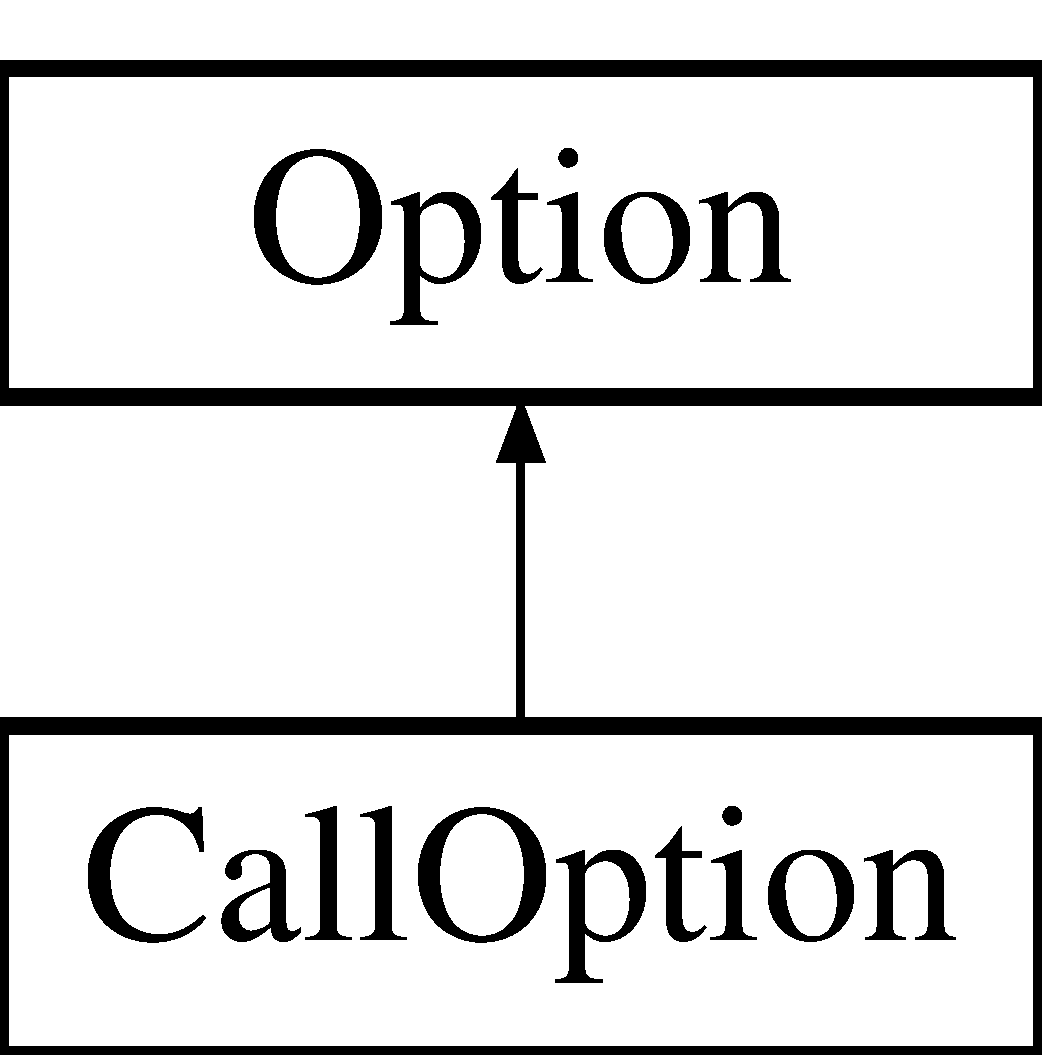
\includegraphics[height=2.000000cm]{classCallOption}
\end{center}
\end{figure}
\subsection*{Public Member Functions}
\begin{DoxyCompactItemize}
\item 
\hyperlink{classCallOption_a6a7af19aa666f2a24318dda2c232654c}{Call\-Option} (double T, int nb\-Time\-Steps, int size, Pnl\-Vect $\ast$weights, double strike)
\item 
double \hyperlink{classCallOption_add068157dca472105aede4a613970dfc}{payoff} (const Pnl\-Mat $\ast$path) override
\end{DoxyCompactItemize}
\subsection*{Public Attributes}
\begin{DoxyCompactItemize}
\item 
double \hyperlink{classCallOption_a5158e7f6be0b959b51e2e92172a49ebf}{strike\-\_\-}
\end{DoxyCompactItemize}


\subsection{Detailed Description}
\hyperlink{classOption}{Option} Call hérite de la classe abstraite option. 

\subsection{Constructor \& Destructor Documentation}
\hypertarget{classCallOption_a6a7af19aa666f2a24318dda2c232654c}{\index{Call\-Option@{Call\-Option}!Call\-Option@{Call\-Option}}
\index{Call\-Option@{Call\-Option}!CallOption@{Call\-Option}}
\subsubsection[{Call\-Option}]{\setlength{\rightskip}{0pt plus 5cm}Call\-Option\-::\-Call\-Option (
\begin{DoxyParamCaption}
\item[{double}]{T, }
\item[{int}]{nb\-Time\-Steps, }
\item[{int}]{size, }
\item[{Pnl\-Vect $\ast$}]{weights, }
\item[{double}]{strike}
\end{DoxyParamCaption}
)}}\label{classCallOption_a6a7af19aa666f2a24318dda2c232654c}
Constructeur de la classe 
\begin{DoxyParams}[1]{Parameters}
\mbox{\tt in}  & {\em T} & \-: maturité \\
\hline
\mbox{\tt in}  & {\em nb\-Time\-Steps} & \-: nombre de pas de temps de discrétisation \\
\hline
\mbox{\tt in}  & {\em size} & \-: dimension du modèle \\
\hline
\mbox{\tt in}  & {\em weights} & \-: poids des actifs \\
\hline
\mbox{\tt in}  & {\em strike} & \-: prix d'exercice de l'option \\
\hline
\end{DoxyParams}


\subsection{Member Function Documentation}
\hypertarget{classCallOption_add068157dca472105aede4a613970dfc}{\index{Call\-Option@{Call\-Option}!payoff@{payoff}}
\index{payoff@{payoff}!CallOption@{Call\-Option}}
\subsubsection[{payoff}]{\setlength{\rightskip}{0pt plus 5cm}double Call\-Option\-::payoff (
\begin{DoxyParamCaption}
\item[{const Pnl\-Mat $\ast$}]{path}
\end{DoxyParamCaption}
)\hspace{0.3cm}{\ttfamily [override]}, {\ttfamily [virtual]}}}\label{classCallOption_add068157dca472105aede4a613970dfc}
Calcule la valeur du payoff sur la trajectoire


\begin{DoxyParams}[1]{Parameters}
\mbox{\tt in}  & {\em path} & est une matrice de taille (N+1) x d contenant une trajectoire du modèle telle que créée par la fonction asset. \\
\hline
\end{DoxyParams}
\begin{DoxyReturn}{Returns}
phi(trajectoire) 
\end{DoxyReturn}


Implements \hyperlink{classOption_abe90882a11f5436077425249e3f32204}{Option}.



\subsection{Member Data Documentation}
\hypertarget{classCallOption_a5158e7f6be0b959b51e2e92172a49ebf}{\index{Call\-Option@{Call\-Option}!strike\-\_\-@{strike\-\_\-}}
\index{strike\-\_\-@{strike\-\_\-}!CallOption@{Call\-Option}}
\subsubsection[{strike\-\_\-}]{\setlength{\rightskip}{0pt plus 5cm}double Call\-Option\-::strike\-\_\-}}\label{classCallOption_a5158e7f6be0b959b51e2e92172a49ebf}
Prix d'exercice de l'option Call 

The documentation for this class was generated from the following files\-:\begin{DoxyCompactItemize}
\item 
/user/5/.\-base/mazarsa/home/3a/calcul\-\_\-parallèle/projet/pricer/chamilo/pricer-\/skel/src/Call\-Option.\-hpp\item 
/user/5/.\-base/mazarsa/home/3a/calcul\-\_\-parallèle/projet/pricer/chamilo/pricer-\/skel/src/Call\-Option.\-cpp\end{DoxyCompactItemize}

\hypertarget{classMonteCarlo}{\section{Monte\-Carlo Class Reference}
\label{classMonteCarlo}\index{Monte\-Carlo@{Monte\-Carlo}}
}


Méthode de Monte Carlo pour les calculs.  




{\ttfamily \#include $<$Monte\-Carlo.\-hpp$>$}

\subsection*{Public Member Functions}
\begin{DoxyCompactItemize}
\item 
\hyperlink{classMonteCarlo_a01b66bd9e983f9adc235bd80c1c544bd}{Monte\-Carlo} (\hyperlink{classBlackScholesModel}{Black\-Scholes\-Model} $\ast$mod, \hyperlink{classOption}{Option} $\ast$opt, Pnl\-Rng $\ast$rng, double fd\-Step, int nb\-Samples)
\item 
void \hyperlink{classMonteCarlo_a5979d4378e3f28878152a310d8a1f7bf}{price} (double \&prix, double \&ic)
\item 
void \hyperlink{classMonteCarlo_aa7bfce4384323c697d0b06840ad3140f}{price} (const Pnl\-Mat $\ast$past, double t, double \&prix, double \&ic)
\item 
void \hyperlink{classMonteCarlo_a6f495c9330ab7ce8f54e1b6ccb516115}{delta} (const Pnl\-Mat $\ast$past, double t, Pnl\-Vect $\ast$delta, Pnl\-Vect $\ast$conf\-\_\-delta)
\item 
void \hyperlink{classMonteCarlo_adb880ac4788d185d305d35270fa00610}{Price\-Delta} (Pnl\-Vect $\ast$list\-Price, Pnl\-Mat $\ast$mat\-Delta, Pnl\-Mat $\ast$market\-Price, int H)
\item 
void \hyperlink{classMonteCarlo_aa2eadab1f496f4c225ceaee9d3b2a37c}{list\-Hedge} (Pnl\-Vect $\ast$list\-Hedge, Pnl\-Vect $\ast$last\-Delta, double \&last\-Price, Pnl\-Mat $\ast$market\-Price)
\item 
void \hyperlink{classMonteCarlo_a1eee6066b282022752e6fb848c49b56c}{pnl} (double \&pnl, Pnl\-Mat $\ast$market\-Price, int H)
\end{DoxyCompactItemize}
\subsection*{Public Attributes}
\begin{DoxyCompactItemize}
\item 
\hyperlink{classBlackScholesModel}{Black\-Scholes\-Model} $\ast$ \hyperlink{classMonteCarlo_a704c29cd8aa027ab01cc556d37c9a764}{mod\-\_\-}
\item 
\hyperlink{classOption}{Option} $\ast$ \hyperlink{classMonteCarlo_af0ee580b0eb87f57c7a41cd2a9e6fc6a}{opt\-\_\-}
\item 
Pnl\-Rng $\ast$ \hyperlink{classMonteCarlo_aa41318b565311457e04383047d68936e}{rng\-\_\-}
\item 
double \hyperlink{classMonteCarlo_a87640dad0fffa3c38d70c8be6c8d61cb}{fd\-Step\-\_\-}
\item 
size\-\_\-t \hyperlink{classMonteCarlo_ad5d0c7f98614e762f6d807e397415c63}{nb\-Samples\-\_\-}
\end{DoxyCompactItemize}


\subsection{Detailed Description}
Méthode de Monte Carlo pour les calculs. 

\subsection{Constructor \& Destructor Documentation}
\hypertarget{classMonteCarlo_a01b66bd9e983f9adc235bd80c1c544bd}{\index{Monte\-Carlo@{Monte\-Carlo}!Monte\-Carlo@{Monte\-Carlo}}
\index{Monte\-Carlo@{Monte\-Carlo}!MonteCarlo@{Monte\-Carlo}}
\subsubsection[{Monte\-Carlo}]{\setlength{\rightskip}{0pt plus 5cm}Monte\-Carlo\-::\-Monte\-Carlo (
\begin{DoxyParamCaption}
\item[{{\bf Black\-Scholes\-Model} $\ast$}]{mod, }
\item[{{\bf Option} $\ast$}]{opt, }
\item[{Pnl\-Rng $\ast$}]{rng, }
\item[{double}]{fd\-Step, }
\item[{int}]{nb\-Samples}
\end{DoxyParamCaption}
)}}\label{classMonteCarlo_a01b66bd9e983f9adc235bd80c1c544bd}
Constructeur de la classe param\mbox{[}in\mbox{]} mod \-: pointeur vers le modèle param\mbox{[}in\mbox{]} opt \-: pointeur sur l'option param\mbox{[}in\mbox{]} rng \-: pointeur sur le générateur param\mbox{[}in\mbox{]} fd\-Step \-: pas de différence finie param\mbox{[}in\mbox{]} nb\-Samples \-: nombre de tirages Monte Carlo 

\subsection{Member Function Documentation}
\hypertarget{classMonteCarlo_a6f495c9330ab7ce8f54e1b6ccb516115}{\index{Monte\-Carlo@{Monte\-Carlo}!delta@{delta}}
\index{delta@{delta}!MonteCarlo@{Monte\-Carlo}}
\subsubsection[{delta}]{\setlength{\rightskip}{0pt plus 5cm}void Monte\-Carlo\-::delta (
\begin{DoxyParamCaption}
\item[{const Pnl\-Mat $\ast$}]{past, }
\item[{double}]{t, }
\item[{Pnl\-Vect $\ast$}]{delta, }
\item[{Pnl\-Vect $\ast$}]{conf\-\_\-delta}
\end{DoxyParamCaption}
)}}\label{classMonteCarlo_a6f495c9330ab7ce8f54e1b6ccb516115}
Calcule le delta de l'option à la date t


\begin{DoxyParams}[1]{Parameters}
\mbox{\tt in}  & {\em past} & contient la trajectoire du sous-\/jacent jusqu'à l'instant t \\
\hline
\mbox{\tt in}  & {\em t} & date à laquelle le calcul est fait \\
\hline
\mbox{\tt out}  & {\em delta} & contient le vecteur de delta \\
\hline
\mbox{\tt in}  & {\em conf\-\_\-delta} & contient le vecteur d'intervalle de confiance sur le calcul du delta \\
\hline
\end{DoxyParams}
\hypertarget{classMonteCarlo_aa2eadab1f496f4c225ceaee9d3b2a37c}{\index{Monte\-Carlo@{Monte\-Carlo}!list\-Hedge@{list\-Hedge}}
\index{list\-Hedge@{list\-Hedge}!MonteCarlo@{Monte\-Carlo}}
\subsubsection[{list\-Hedge}]{\setlength{\rightskip}{0pt plus 5cm}void Monte\-Carlo\-::list\-Hedge (
\begin{DoxyParamCaption}
\item[{Pnl\-Vect $\ast$}]{list\-Hedge, }
\item[{Pnl\-Vect $\ast$}]{last\-Delta, }
\item[{double \&}]{last\-Price, }
\item[{Pnl\-Mat $\ast$}]{market\-Price}
\end{DoxyParamCaption}
)}}\label{classMonteCarlo_aa2eadab1f496f4c225ceaee9d3b2a37c}
Construction du portefeuille de couverture Calcul de l'évolution de la part investie au taux sans risque


\begin{DoxyParams}[1]{Parameters}
\mbox{\tt out}  & {\em list\-Hedge} & contient la valeur du portefeuille de couverture à differents instants \\
\hline
\mbox{\tt in}  & {\em market\-Price} & contient la disposition des trajectoires de marché \\
\hline
\mbox{\tt in}  & {\em last\-Delta} & delta dernier instant (a maturite) \\
\hline
\mbox{\tt in}  & {\em last\-Price} & delta dernier instant (a maturite)\\
\hline
\end{DoxyParams}
Construction du portefeuille de couverture Calcul de l'évolution de la part investie au taux sans risque


\begin{DoxyParams}[1]{Parameters}
\mbox{\tt out}  & {\em list\-Hedge} & contient la valeur du portefeuille de couverture à differents instants \\
\hline
\mbox{\tt in}  & {\em market\-Price} & contient la disposition des trajectoires de marché \\
\hline
\end{DoxyParams}
\hypertarget{classMonteCarlo_a1eee6066b282022752e6fb848c49b56c}{\index{Monte\-Carlo@{Monte\-Carlo}!pnl@{pnl}}
\index{pnl@{pnl}!MonteCarlo@{Monte\-Carlo}}
\subsubsection[{pnl}]{\setlength{\rightskip}{0pt plus 5cm}void Monte\-Carlo\-::pnl (
\begin{DoxyParamCaption}
\item[{double \&}]{pnl, }
\item[{Pnl\-Mat $\ast$}]{market\-Price, }
\item[{int}]{H}
\end{DoxyParamCaption}
)}}\label{classMonteCarlo_a1eee6066b282022752e6fb848c49b56c}
Profit and Loss Calcul de l'erreur de couverture 
\begin{DoxyParams}[1]{Parameters}
\mbox{\tt out}  & {\em pnl} & \-: erreur de couverture \\
\hline
\mbox{\tt in}  & {\em market\-Price} & \-: disposition des trajectoires de marché \\
\hline
\mbox{\tt in}  & {\em H} & \-: nombre de rebalancements \\
\hline
\end{DoxyParams}
\hypertarget{classMonteCarlo_a5979d4378e3f28878152a310d8a1f7bf}{\index{Monte\-Carlo@{Monte\-Carlo}!price@{price}}
\index{price@{price}!MonteCarlo@{Monte\-Carlo}}
\subsubsection[{price}]{\setlength{\rightskip}{0pt plus 5cm}void Monte\-Carlo\-::price (
\begin{DoxyParamCaption}
\item[{double \&}]{prix, }
\item[{double \&}]{ic}
\end{DoxyParamCaption}
)}}\label{classMonteCarlo_a5979d4378e3f28878152a310d8a1f7bf}
Calcule le prix de l'option à la date 0


\begin{DoxyParams}[1]{Parameters}
\mbox{\tt out}  & {\em prix} & valeur de l'estimateur Monte Carlo \\
\hline
\mbox{\tt out}  & {\em ic} & largeur de l'intervalle de confiance \\
\hline
\end{DoxyParams}
\hypertarget{classMonteCarlo_aa7bfce4384323c697d0b06840ad3140f}{\index{Monte\-Carlo@{Monte\-Carlo}!price@{price}}
\index{price@{price}!MonteCarlo@{Monte\-Carlo}}
\subsubsection[{price}]{\setlength{\rightskip}{0pt plus 5cm}void Monte\-Carlo\-::price (
\begin{DoxyParamCaption}
\item[{const Pnl\-Mat $\ast$}]{past, }
\item[{double}]{t, }
\item[{double \&}]{prix, }
\item[{double \&}]{ic}
\end{DoxyParamCaption}
)}}\label{classMonteCarlo_aa7bfce4384323c697d0b06840ad3140f}
Calcule le prix de l'option à la date t


\begin{DoxyParams}[1]{Parameters}
\mbox{\tt in}  & {\em past} & contient la trajectoire du sous-\/jacent jusqu'à l'instant t \\
\hline
\mbox{\tt in}  & {\em t} & date à laquelle le calcul est fait \\
\hline
\mbox{\tt out}  & {\em prix} & contient le prix \\
\hline
\mbox{\tt out}  & {\em ic} & contient la largeur de l'intervalle de confiance sur le calcul du prix \\
\hline
\end{DoxyParams}
\hypertarget{classMonteCarlo_adb880ac4788d185d305d35270fa00610}{\index{Monte\-Carlo@{Monte\-Carlo}!Price\-Delta@{Price\-Delta}}
\index{Price\-Delta@{Price\-Delta}!MonteCarlo@{Monte\-Carlo}}
\subsubsection[{Price\-Delta}]{\setlength{\rightskip}{0pt plus 5cm}void Monte\-Carlo\-::\-Price\-Delta (
\begin{DoxyParamCaption}
\item[{Pnl\-Vect $\ast$}]{list\-Price, }
\item[{Pnl\-Mat $\ast$}]{mat\-Delta, }
\item[{Pnl\-Mat $\ast$}]{market\-Price, }
\item[{int}]{H}
\end{DoxyParamCaption}
)}}\label{classMonteCarlo_adb880ac4788d185d305d35270fa00610}
Calcule le prix et le delta des options à tout instant donné


\begin{DoxyParams}[1]{Parameters}
\mbox{\tt out}  & {\em list\-Price} & contient le prix des options à differents instants \\
\hline
\mbox{\tt in}  & {\em mat\-Delta} & contient le delta des options à differents instants \\
\hline
\mbox{\tt in}  & {\em market\-Price} & contient la disposition des trajectoires de marché \\
\hline
\mbox{\tt in}  & {\em H} & \-: nombre de rebalancements \\
\hline
\end{DoxyParams}


\subsection{Member Data Documentation}
\hypertarget{classMonteCarlo_a87640dad0fffa3c38d70c8be6c8d61cb}{\index{Monte\-Carlo@{Monte\-Carlo}!fd\-Step\-\_\-@{fd\-Step\-\_\-}}
\index{fd\-Step\-\_\-@{fd\-Step\-\_\-}!MonteCarlo@{Monte\-Carlo}}
\subsubsection[{fd\-Step\-\_\-}]{\setlength{\rightskip}{0pt plus 5cm}double Monte\-Carlo\-::fd\-Step\-\_\-}}\label{classMonteCarlo_a87640dad0fffa3c38d70c8be6c8d61cb}
pas de h \hypertarget{classMonteCarlo_a704c29cd8aa027ab01cc556d37c9a764}{\index{Monte\-Carlo@{Monte\-Carlo}!mod\-\_\-@{mod\-\_\-}}
\index{mod\-\_\-@{mod\-\_\-}!MonteCarlo@{Monte\-Carlo}}
\subsubsection[{mod\-\_\-}]{\setlength{\rightskip}{0pt plus 5cm}{\bf Black\-Scholes\-Model}$\ast$ Monte\-Carlo\-::mod\-\_\-}}\label{classMonteCarlo_a704c29cd8aa027ab01cc556d37c9a764}
pointeur vers le modèle de Black Scholes \hypertarget{classMonteCarlo_ad5d0c7f98614e762f6d807e397415c63}{\index{Monte\-Carlo@{Monte\-Carlo}!nb\-Samples\-\_\-@{nb\-Samples\-\_\-}}
\index{nb\-Samples\-\_\-@{nb\-Samples\-\_\-}!MonteCarlo@{Monte\-Carlo}}
\subsubsection[{nb\-Samples\-\_\-}]{\setlength{\rightskip}{0pt plus 5cm}size\-\_\-t Monte\-Carlo\-::nb\-Samples\-\_\-}}\label{classMonteCarlo_ad5d0c7f98614e762f6d807e397415c63}
nombre de tirages Monte Carlo \hypertarget{classMonteCarlo_af0ee580b0eb87f57c7a41cd2a9e6fc6a}{\index{Monte\-Carlo@{Monte\-Carlo}!opt\-\_\-@{opt\-\_\-}}
\index{opt\-\_\-@{opt\-\_\-}!MonteCarlo@{Monte\-Carlo}}
\subsubsection[{opt\-\_\-}]{\setlength{\rightskip}{0pt plus 5cm}{\bf Option}$\ast$ Monte\-Carlo\-::opt\-\_\-}}\label{classMonteCarlo_af0ee580b0eb87f57c7a41cd2a9e6fc6a}
pointeur sur l'option \hypertarget{classMonteCarlo_aa41318b565311457e04383047d68936e}{\index{Monte\-Carlo@{Monte\-Carlo}!rng\-\_\-@{rng\-\_\-}}
\index{rng\-\_\-@{rng\-\_\-}!MonteCarlo@{Monte\-Carlo}}
\subsubsection[{rng\-\_\-}]{\setlength{\rightskip}{0pt plus 5cm}Pnl\-Rng$\ast$ Monte\-Carlo\-::rng\-\_\-}}\label{classMonteCarlo_aa41318b565311457e04383047d68936e}
pointeur sur le générateur de nombres aléatoires 

The documentation for this class was generated from the following files\-:\begin{DoxyCompactItemize}
\item 
/user/5/.\-base/mazarsa/home/3a/calcul\-\_\-parallèle/projet/pricer/chamilo/pricer-\/skel/src/Monte\-Carlo.\-hpp\item 
/user/5/.\-base/mazarsa/home/3a/calcul\-\_\-parallèle/projet/pricer/chamilo/pricer-\/skel/src/Monte\-Carlo.\-cpp\end{DoxyCompactItemize}

\hypertarget{classOption}{\section{Option Class Reference}
\label{classOption}\index{Option@{Option}}
}


Classe \hyperlink{classOption}{Option} abstraite.  




{\ttfamily \#include $<$Option.\-hpp$>$}

Inheritance diagram for Option\-:\begin{figure}[H]
\begin{center}
\leavevmode
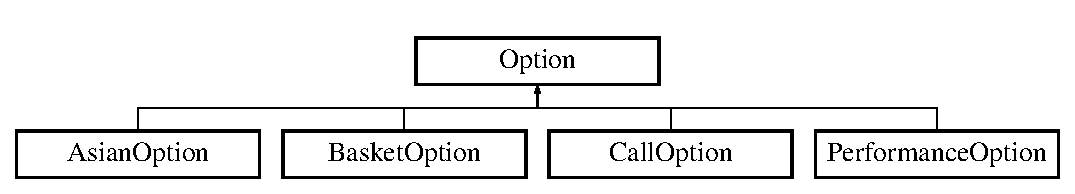
\includegraphics[height=2.000000cm]{classOption}
\end{center}
\end{figure}
\subsection*{Public Member Functions}
\begin{DoxyCompactItemize}
\item 
virtual double \hyperlink{classOption_abe90882a11f5436077425249e3f32204}{payoff} (const Pnl\-Mat $\ast$path)=0
\end{DoxyCompactItemize}
\subsection*{Public Attributes}
\begin{DoxyCompactItemize}
\item 
double \hyperlink{classOption_a89f0365b68626cc5eb523f12159e0764}{T\-\_\-}
\item 
int \hyperlink{classOption_ad424223ea2698144e823c494d625fbe0}{nb\-Time\-Steps\-\_\-}
\item 
int \hyperlink{classOption_a65fae5103b50f953f29a86b1a17b4540}{size\-\_\-}
\item 
Pnl\-Vect $\ast$ \hyperlink{classOption_a8f5978de54bbccdc3af36f30eaae1fdb}{weights\-\_\-}
\end{DoxyCompactItemize}


\subsection{Detailed Description}
Classe \hyperlink{classOption}{Option} abstraite. 

\subsection{Member Function Documentation}
\hypertarget{classOption_abe90882a11f5436077425249e3f32204}{\index{Option@{Option}!payoff@{payoff}}
\index{payoff@{payoff}!Option@{Option}}
\subsubsection[{payoff}]{\setlength{\rightskip}{0pt plus 5cm}virtual double Option\-::payoff (
\begin{DoxyParamCaption}
\item[{const Pnl\-Mat $\ast$}]{path}
\end{DoxyParamCaption}
)\hspace{0.3cm}{\ttfamily [pure virtual]}}}\label{classOption_abe90882a11f5436077425249e3f32204}
Calcule la valeur du payoff sur la trajectoire


\begin{DoxyParams}[1]{Parameters}
\mbox{\tt in}  & {\em path} & est une matrice de taille (N+1) x d contenant une trajectoire du modèle telle que créée par la fonction asset. \\
\hline
\end{DoxyParams}
\begin{DoxyReturn}{Returns}
phi(trajectoire) 
\end{DoxyReturn}


Implemented in \hyperlink{classAsianOption_a0ac88380a30a7c0ef6a5c5159d15fa76}{Asian\-Option}, \hyperlink{classBasketOption_a57c941403d2bd21159b090fa6481ee9e}{Basket\-Option}, \hyperlink{classCallOption_add068157dca472105aede4a613970dfc}{Call\-Option}, and \hyperlink{classPerformanceOption_ad1effaaa7b93de07b5add0805c070bc7}{Performance\-Option}.



\subsection{Member Data Documentation}
\hypertarget{classOption_ad424223ea2698144e823c494d625fbe0}{\index{Option@{Option}!nb\-Time\-Steps\-\_\-@{nb\-Time\-Steps\-\_\-}}
\index{nb\-Time\-Steps\-\_\-@{nb\-Time\-Steps\-\_\-}!Option@{Option}}
\subsubsection[{nb\-Time\-Steps\-\_\-}]{\setlength{\rightskip}{0pt plus 5cm}int Option\-::nb\-Time\-Steps\-\_\-}}\label{classOption_ad424223ea2698144e823c494d625fbe0}
nombre de pas de temps de discrétisation \hypertarget{classOption_a65fae5103b50f953f29a86b1a17b4540}{\index{Option@{Option}!size\-\_\-@{size\-\_\-}}
\index{size\-\_\-@{size\-\_\-}!Option@{Option}}
\subsubsection[{size\-\_\-}]{\setlength{\rightskip}{0pt plus 5cm}int Option\-::size\-\_\-}}\label{classOption_a65fae5103b50f953f29a86b1a17b4540}
dimension du modèle, redondant avec \hyperlink{classBlackScholesModel_ab84e9318c0c1e8a50d5e2f9a70f1256e}{Black\-Scholes\-Model\-::size\-\_\-} \hypertarget{classOption_a89f0365b68626cc5eb523f12159e0764}{\index{Option@{Option}!T\-\_\-@{T\-\_\-}}
\index{T\-\_\-@{T\-\_\-}!Option@{Option}}
\subsubsection[{T\-\_\-}]{\setlength{\rightskip}{0pt plus 5cm}double Option\-::\-T\-\_\-}}\label{classOption_a89f0365b68626cc5eb523f12159e0764}
maturité de l'option \hypertarget{classOption_a8f5978de54bbccdc3af36f30eaae1fdb}{\index{Option@{Option}!weights\-\_\-@{weights\-\_\-}}
\index{weights\-\_\-@{weights\-\_\-}!Option@{Option}}
\subsubsection[{weights\-\_\-}]{\setlength{\rightskip}{0pt plus 5cm}Pnl\-Vect$\ast$ Option\-::weights\-\_\-}}\label{classOption_a8f5978de54bbccdc3af36f30eaae1fdb}
poids des sous-\/jacents 

The documentation for this class was generated from the following file\-:\begin{DoxyCompactItemize}
\item 
/user/5/.\-base/mazarsa/home/3a/calcul\-\_\-parallèle/projet/pricer/chamilo/pricer-\/skel/src/Option.\-hpp\end{DoxyCompactItemize}

\hypertarget{classPerformanceOption}{\section{Performance\-Option Class Reference}
\label{classPerformanceOption}\index{Performance\-Option@{Performance\-Option}}
}


\hyperlink{classOption}{Option} Performance hérite de la classe abstraite option.  




{\ttfamily \#include $<$Performance\-Option.\-hpp$>$}

Inheritance diagram for Performance\-Option\-:\begin{figure}[H]
\begin{center}
\leavevmode
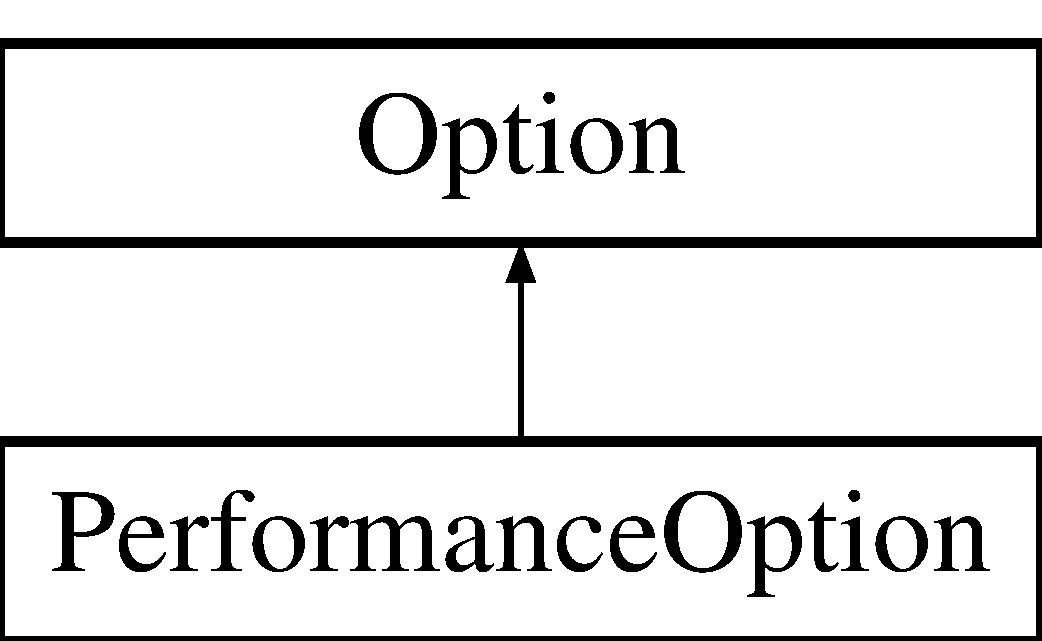
\includegraphics[height=2.000000cm]{classPerformanceOption}
\end{center}
\end{figure}
\subsection*{Public Member Functions}
\begin{DoxyCompactItemize}
\item 
\hyperlink{classPerformanceOption_a2bee53d8bcc5cf42fbe9c1144985eea1}{Performance\-Option} (double T, int nb\-Time\-Steps, int size, Pnl\-Vect $\ast$weights)
\item 
double \hyperlink{classPerformanceOption_ad1effaaa7b93de07b5add0805c070bc7}{payoff} (const Pnl\-Mat $\ast$path) override
\end{DoxyCompactItemize}
\subsection*{Additional Inherited Members}


\subsection{Detailed Description}
\hyperlink{classOption}{Option} Performance hérite de la classe abstraite option. 

\subsection{Constructor \& Destructor Documentation}
\hypertarget{classPerformanceOption_a2bee53d8bcc5cf42fbe9c1144985eea1}{\index{Performance\-Option@{Performance\-Option}!Performance\-Option@{Performance\-Option}}
\index{Performance\-Option@{Performance\-Option}!PerformanceOption@{Performance\-Option}}
\subsubsection[{Performance\-Option}]{\setlength{\rightskip}{0pt plus 5cm}Performance\-Option\-::\-Performance\-Option (
\begin{DoxyParamCaption}
\item[{double}]{T, }
\item[{int}]{nb\-Time\-Steps, }
\item[{int}]{size, }
\item[{Pnl\-Vect $\ast$}]{weights}
\end{DoxyParamCaption}
)}}\label{classPerformanceOption_a2bee53d8bcc5cf42fbe9c1144985eea1}
Constructeur de la classe 
\begin{DoxyParams}[1]{Parameters}
\mbox{\tt in}  & {\em T} & \-: maturité \\
\hline
\mbox{\tt in}  & {\em nb\-Time\-Steps} & \-: nombre de pas de temps de discrétisation \\
\hline
\mbox{\tt in}  & {\em size} & \-: dimension du modèle \\
\hline
\mbox{\tt in}  & {\em weights} & \-: poids des actifs \\
\hline
\end{DoxyParams}


\subsection{Member Function Documentation}
\hypertarget{classPerformanceOption_ad1effaaa7b93de07b5add0805c070bc7}{\index{Performance\-Option@{Performance\-Option}!payoff@{payoff}}
\index{payoff@{payoff}!PerformanceOption@{Performance\-Option}}
\subsubsection[{payoff}]{\setlength{\rightskip}{0pt plus 5cm}double Performance\-Option\-::payoff (
\begin{DoxyParamCaption}
\item[{const Pnl\-Mat $\ast$}]{path}
\end{DoxyParamCaption}
)\hspace{0.3cm}{\ttfamily [override]}, {\ttfamily [virtual]}}}\label{classPerformanceOption_ad1effaaa7b93de07b5add0805c070bc7}
Calcule la valeur du payoff sur la trajectoire


\begin{DoxyParams}[1]{Parameters}
\mbox{\tt in}  & {\em path} & est une matrice de taille (N+1) x d contenant une trajectoire du modèle telle que créée par la fonction asset. \\
\hline
\end{DoxyParams}
\begin{DoxyReturn}{Returns}
phi(trajectoire) 
\end{DoxyReturn}


Implements \hyperlink{classOption_abe90882a11f5436077425249e3f32204}{Option}.



The documentation for this class was generated from the following files\-:\begin{DoxyCompactItemize}
\item 
/user/5/.\-base/mazarsa/home/3a/calcul\-\_\-parallèle/projet/pricer/chamilo/pricer-\/skel/src/Performance\-Option.\-hpp\item 
/user/5/.\-base/mazarsa/home/3a/calcul\-\_\-parallèle/projet/pricer/chamilo/pricer-\/skel/src/Performance\-Option.\-cpp\end{DoxyCompactItemize}

%--- End generated contents ---

% Index
\newpage
\phantomsection
\addcontentsline{toc}{part}{Index}
\printindex

\end{document}
